\documentclass[12pt]{article}
\usepackage[utf8]{inputenc}
\usepackage[spanish]{babel}
\decimalpoint
\usepackage{amsmath}
\usepackage{caption}
\usepackage{amsthm}
\usepackage{amssymb}
\usepackage{graphicx}
\usepackage[margin=0.9in]{geometry}
\usepackage{fancyhdr}
\usepackage[inline]{enumitem}
\usepackage{float}
\usepackage{cancel}
\usepackage{bigints}
\usepackage{color}
\usepackage{xcolor}
\usepackage{listingsutf8}
\usepackage{algorithm}
\usepackage{tocloft}
\usepackage[none]{hyphenat}
\usepackage{graphicx}
\usepackage{grffile}
\usepackage{tabularx}
\usepackage[nottoc,notlot,notlof]{tocbibind}
\usepackage{times}
\usepackage{color}
\definecolor{gray97}{gray}{.97}
\definecolor{gray75}{gray}{.75}
\definecolor{gray45}{gray}{.45}
\renewcommand{\cftsecleader}{\cftdotfill{\cftdotsep}}
\pagestyle{fancy}
\setlength{\headheight}{15pt} 
\lhead{EJERCICIO 7 - Diseño de soluciones PD}
\rhead{\thepage}
\lfoot{ESCOM-IPN}
\renewcommand{\footrulewidth}{0.5pt}
\setlength{\parskip}{0.5em}
\newcommand{\ve}[1]{\overrightarrow{#1}}
\newcommand{\abs}[1]{\left\lvert #1 \right\lvert}
\date{26 de febrero de 2017}
\title{Pruebas a posteriori}
\author{Reporte 1}

\definecolor{pblue}{rgb}{0.13,0.13,1}
\definecolor{pgreen}{rgb}{0,0.5,0}
\definecolor{pred}{rgb}{0.9,0,0}
\definecolor{pgrey}{rgb}{0.46,0.45,0.48}
\lstset{tabsize=1}

\usepackage{listings}
\lstset{ frame=Ltb,
framerule=0pt,
aboveskip=0.5cm,
framextopmargin=3pt,
framexbottommargin=3pt,
framexleftmargin=0.4cm,
framesep=0pt,
rulesep=.4pt,
backgroundcolor=\color{gray97},
rulesepcolor=\color{black},
%
stringstyle=\ttfamily,
showstringspaces = false,
basicstyle=\small\ttfamily,
commentstyle=\color{gray45},
keywordstyle=\bfseries,
%
numbers=left,
numbersep=15pt,
numberstyle=\tiny,
numberfirstline = false,
breaklines=true,
}

% minimizar fragmentado de listados
\lstnewenvironment{listing}[1][]
{\lstset{#1}\pagebreak[0]}{\pagebreak[0]}

\lstdefinestyle{consola}
{basicstyle=\scriptsize\bf\ttfamily,
backgroundcolor=\color{gray75},
}

\lstdefinestyle{Java}
{language=Java,
}

%%%%%%%%%%%%%%%%%%%%%

\lstdefinestyle{customc}{
  belowcaptionskip=1\baselineskip,
  breaklines=true,
  frame=L,
  xleftmargin=\parindent,
  language=C,
  showstringspaces=false,
  basicstyle=\footnotesize\ttfamily,
  keywordstyle=\bfseries\color{green!40!black},
  commentstyle=\itshape\color{purple!40!black},
  identifierstyle=\color{blue},
  stringstyle=\color{orange},
}

\lstdefinestyle{customasm}{
  belowcaptionskip=1\baselineskip,
  frame=L,
  xleftmargin=\parindent,
  language=[x86masm]Assembler,
  basicstyle=\footnotesize\ttfamily,
  commentstyle=\itshape\color{purple!40!black},
}

\lstset{escapechar=@,style=customc}


    % =====  CODE EDITOR =========
    \lstdefinestyle{CompilandoStyle} {                              %This is Code Style
        backgroundcolor=\color{BlueGrey800MD},                      %Background Color  
        basicstyle=\tiny\color{white},                              %Font color
        commentstyle=\color{BlueGrey100MD},                         %Comment color
        stringstyle=\color{TealMD},                                 %String color
        keywordstyle=\color{Green100MD},                            %keywords color
        numberstyle=\tiny\color{TealMD},                            %Size of a number
        frame=shadowbox,                                            %Adds a frame around the code
        breakatwhitespace=true,                                     %Style                       
        breaklines=true,                                            %Style                   
        keepspaces=true,                                            %Style                   
        numbers=left,                                               %Style                   
        numbersep=10pt,                                             %Style 
        xleftmargin=\parindent,                                     %Style 
        tabsize=4                                                   %Style 
    }
 
    \lstset{style=CompilandoStyle}                                  %Use this style

    \usepackage{minted} % Paquete que permite citar codigo
    \usemintedstyle{borland} % Aqui se define el colorscheme para minted
    \setminted{
        fontsize = \scriptsize, % Ajusta el codigo a la hoja
        baselinestretch = 1,
        linenos, % set numbers
        breaklines=true, % Hace un salto de linea automatico en caso de que se llege al final de la line
        tabsize=3 
    }

%Permite crear columnas en el documento
\usepackage{multicol} 
\usepackage{color}
\usepackage{comment}
\newcommand{\tabitem}{~~\llap{\textbullet}~~}
\newcommand{\subtabitem}{~~~~\llap{\textbullet}~~}

% ---------------------------------------------------
%                       FONT 
% ---------------------------------------------------

\usepackage{cmbright}                               % Font


\begin{document}

% ###########################################################################################
% ----------------------------------- FANCY TITLE PAGE --------------------------------------
% ###########################################################################################
\begin{titlepage}
            \begin{center}
                \noindent
                \begin{minipage}{0.5\textwidth}
                    \begin{flushleft} \large
                        \includegraphics[width=0.3\textwidth]{../ipn.png}
                    \end{flushleft}
                \end{minipage}%
                \begin{minipage}{0.55\textwidth}
                    \begin{flushright} \large
                        \includegraphics[width=0.5\textwidth]{../escom.png}
                    \end{flushright}
                \end{minipage}
                
                \textsc{\LARGE Instituto Politécnico Nacional}\\[0.5cm]
                
                \textsc{\Large Escuela Superior de Cómputo}\\[1cm]
                
                % Title
                
                { \huge Ejercicio 06 - Diseño de soluciones con Programación Dinámica \\[1cm] }
                
                { \Large Unidad de aprendizaje: Análisis de algoritmos} \\[1cm]
                
                { \Large Grupo: 3CM3 } \\[1cm]
                
                \noindent
                \begin{minipage}{0.5\textwidth}
                    \begin{flushleft} \large
                        \emph{Alumno(a):}\\
                        
                        \begin{tabular}{ll}
                         Nicolás Sayago Abigail\\
                    \end{tabular}
                    \end{flushleft}
                \end{minipage}%
                \begin{minipage}{0.5\textwidth}
                    \begin{flushright} \large
                        \emph{Profesor(a):} \\
                        Edgardo Adrian Franco  \\
                    \end{flushright}
                \end{minipage}
                \vfill
                \begin{minipage}{0.5\textwidth}
                    \begin{center} \large
                        \includegraphics[width=0.6\textwidth]{Abigail/Images/A.jpg}
                    \end{center}
                \end{minipage}
                    
                % Bottom of the page
                {\large 23 Noviembre de 2018}
            \end{center}
        \end{titlepage}
    \tableofcontents
  \newpage

  \section{Instrucciones}

  Para los siguientes 5 grafos detallar la solución de la ruta más corta del nodo (1 o A) a todos los nodos (Dijkstra) y el árbol recubridor mínimo mediante Prim y Kruskal.

  Describir de manera detallada los algoritmos y sus pasos.

  % -----------------------------------------------
  %                   EJERCICIO 01
  % -----------------------------------------------
  
  \section{Ejercicio 01}

    \begin{figure}[h!]
      \centering
      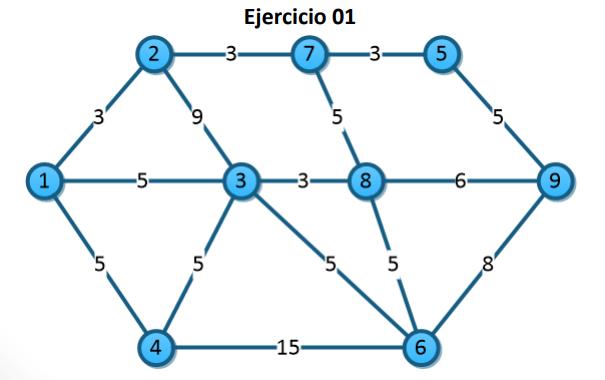
\includegraphics[width=0.7\textwidth]{Abigail/Ejercicio09/Images/1.PNG}
    \end{figure} 

    \subsection{Dijkstra}

      \subsubsection{Tabla}
        Ruta más corta desde el nodo 1 hasta los demás.

        \begin{itemize}
          \item La ruta más costosa: 14 hacia el nodo 14.
        \end{itemize}

        \begin{figure}[h!]
          \centering
          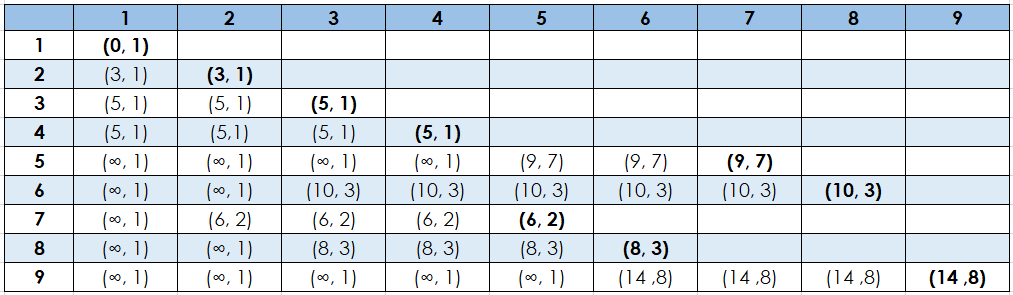
\includegraphics[width=0.7\textwidth]{Abigail/Ejercicio09/Images/1_DT.PNG}
        \end{figure} 

      \subsubsection{Resultado}
        \begin{figure}[h!]
          \centering
          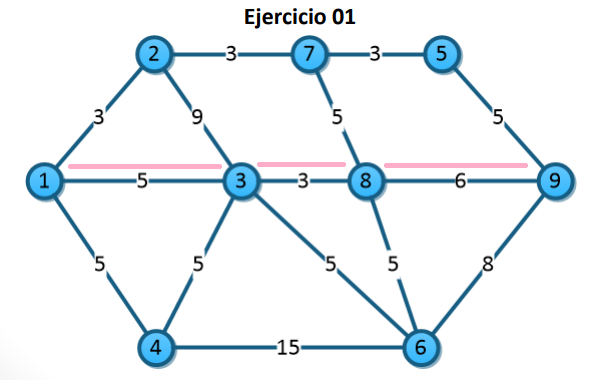
\includegraphics[width=0.7\textwidth]{Abigail/Ejercicio09/Images/1_DR.PNG}
        \end{figure} 


    \subsection{Prim}

      \subsubsection{Explicación}

      \subsubsection{Tabla}
        \begin{figure}[h!]
          \centering
          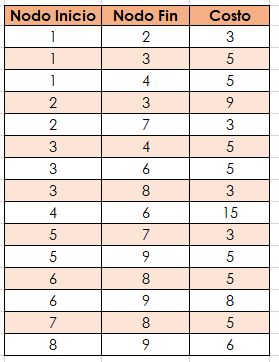
\includegraphics[width=0.7\textwidth]{Abigail/Ejercicio09/Images/1_PT.PNG}
        \end{figure} 

      \subsubsection{Resultado}
        \begin{figure}[h!]
          \centering
          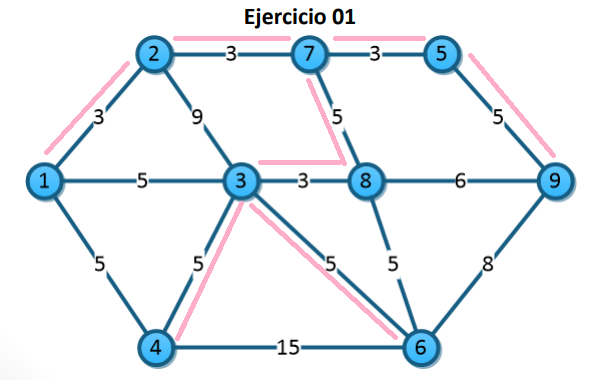
\includegraphics[width=0.7\textwidth]{Abigail/Ejercicio09/Images/1_PR.PNG}
        \end{figure} 

    \subsection{Kruskal}

      \subsubsection{Tabla}

        \begin{figure}[h!]
          \centering
          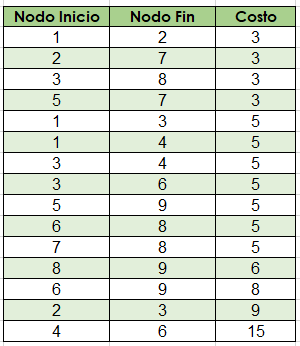
\includegraphics[width=0.7\textwidth]{Abigail/Ejercicio09/Images/1_KT.PNG}
        \end{figure} 

      \subsubsection{Resultado}

        \begin{figure}[h!]
          \centering
          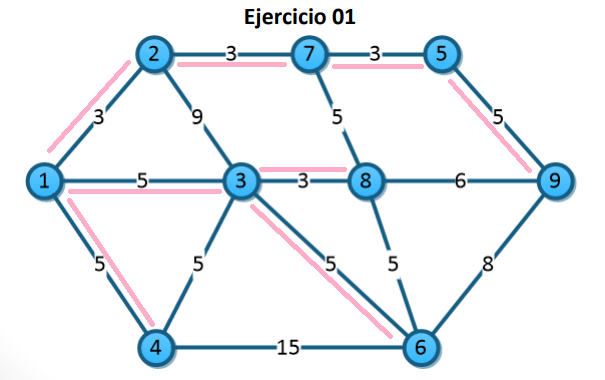
\includegraphics[width=0.7\textwidth]{Abigail/Ejercicio09/Images/1_KR.PNG}
        \end{figure} 


  % -----------------------------------------------
  %                   EJERCICIO 02
  % -----------------------------------------------
  
  \section{Ejercicio 02}

    \begin{figure}[h!]
      \centering
      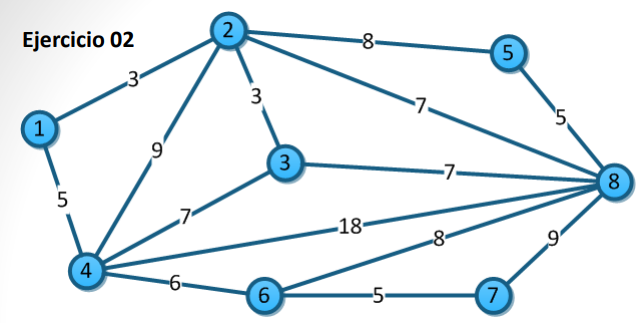
\includegraphics[width=0.7\textwidth]{Abigail/Ejercicio09/Images/2.PNG}
    \end{figure} 

    \subsection{Dijkstra}

      \subsubsection{Tabla}
        Ruta más corta desde el nodo 1 hasta los demás.

        \begin{itemize}
          \item La ruta más costosa: 14 hacia el nodo 14.
        \end{itemize}
        
        \begin{figure}[h!]
          \centering
          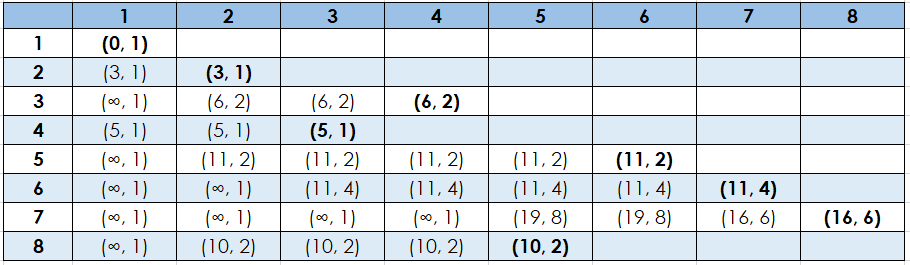
\includegraphics[width=0.7\textwidth]{Abigail/Ejercicio09/Images/2_DT.PNG}
        \end{figure} 

      \subsubsection{Resultado}
        \begin{figure}[h!]
          \centering
          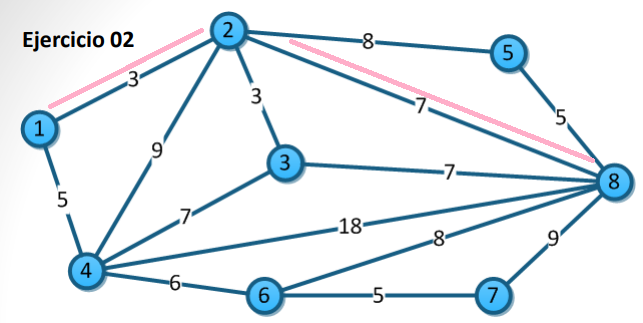
\includegraphics[width=0.7\textwidth]{Abigail/Ejercicio09/Images/2_DR.PNG}
        \end{figure} 


    \subsection{Prim}

      \subsubsection{Explicación}

      \subsubsection{Tabla}

      \subsubsection{Resultado}

    \subsection{Kruskal}

      \subsubsection{Explicación}

      \subsubsection{Tabla}

      \subsubsection{Resultado}

  % -----------------------------------------------
  %                   EJERCICIO 03
  % -----------------------------------------------
  
  \section{Ejercicio 03}
    \begin{figure}[h!]
      \centering
      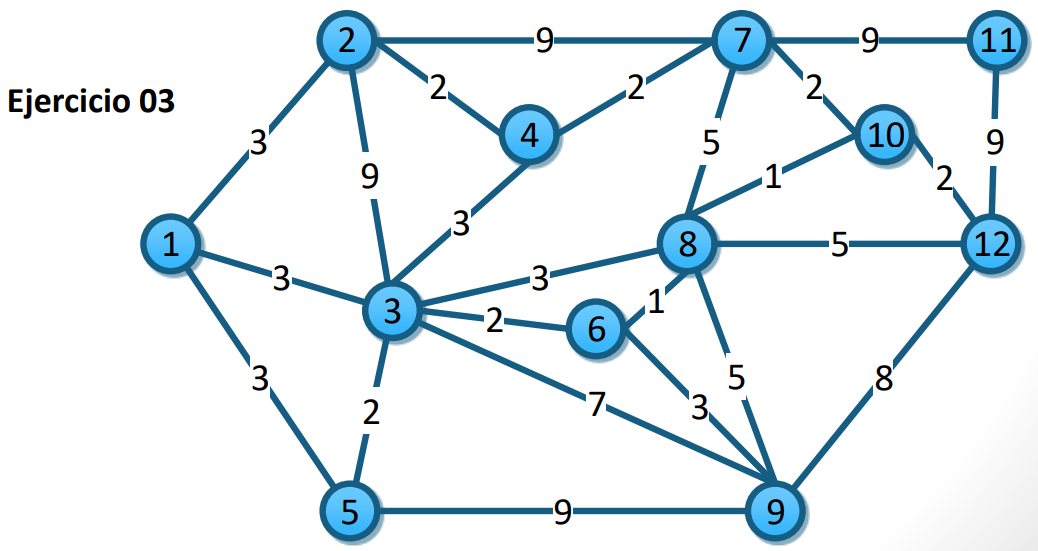
\includegraphics[width=0.7\textwidth]{Abigail/Ejercicio09/Images/3.PNG}
    \end{figure} 

    \subsection{Dijkstra}

      \subsubsection{Tabla}
        Ruta más corta desde el nodo 1 hasta los demás.

        \begin{itemize}
          \item La ruta más costosa: 14 hacia el nodo 14.
        \end{itemize}
        
        \begin{figure}[h!]
          \centering
          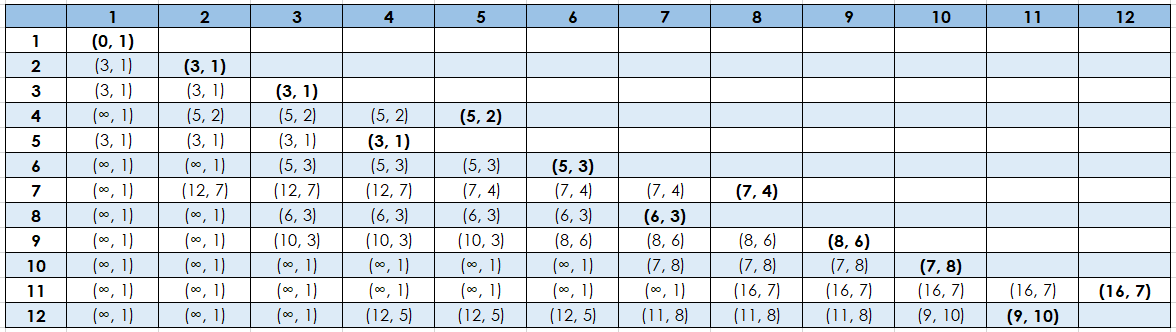
\includegraphics[width=0.7\textwidth]{Abigail/Ejercicio09/Images/3_DT.PNG}
        \end{figure} 

      \subsubsection{Resultado}
        \begin{figure}[h!]
          \centering
          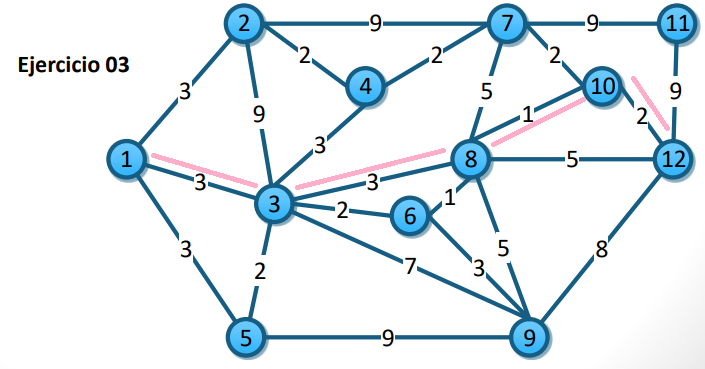
\includegraphics[width=0.7\textwidth]{Abigail/Ejercicio09/Images/3_DR.PNG}
        \end{figure} 


    \subsection{Prim}

      \subsubsection{Tabla}

        Ruta más corta desde el nodo 1 hasta los demás.

        \begin{itemize}
          \item La ruta más costosa: 14 hacia el nodo 14.
        \end{itemize}

      \subsubsection{Resultado}

    \subsection{Kruskal}

      \subsubsection{Explicación}

      \subsubsection{Tabla}

      \subsubsection{Resultado}

  % -----------------------------------------------
  %                   EJERCICIO 04
  % -----------------------------------------------
  
  \section{Ejercicio 04}

    \begin{figure}[h!]
      \centering
      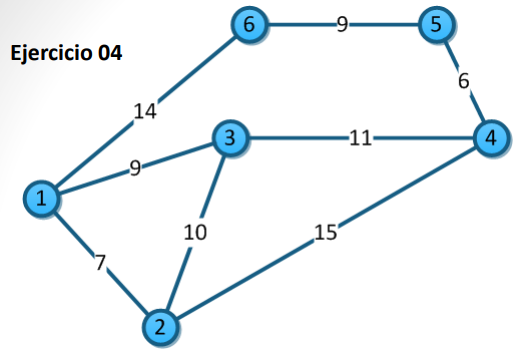
\includegraphics[width=0.7\textwidth]{Abigail/Ejercicio09/Images/4.PNG}
    \end{figure} 

    \subsection{Dijkstra}

      \subsubsection{Tabla}
        Ruta más corta desde el nodo 1 hasta los demás.

        \begin{itemize}
          \item La ruta más costosa: 14 hacia el nodo 14.
        \end{itemize}

        \begin{figure}[h!]
          \centering
          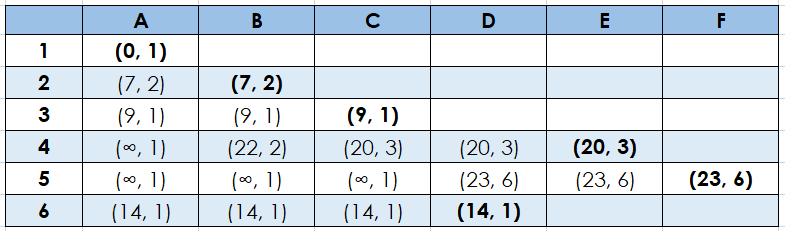
\includegraphics[width=0.7\textwidth]{Abigail/Ejercicio09/Images/4_DT.PNG}
        \end{figure} 

      \subsubsection{Resultado}
        \begin{figure}[h!]
          \centering
          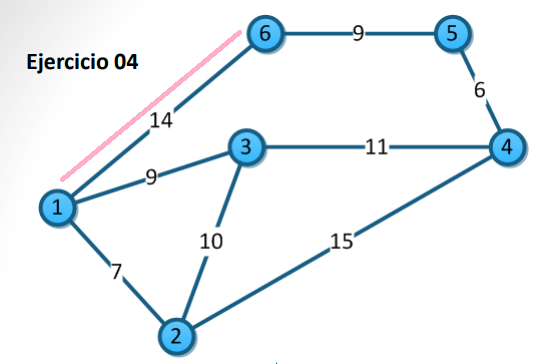
\includegraphics[width=0.7\textwidth]{Abigail/Ejercicio09/Images/4_DR.PNG}
        \end{figure} 

    \subsection{Prim}

      \subsubsection{Explicación}

      \subsubsection{Tabla}

      \subsubsection{Resultado}

    \subsection{Kruskal}

      \subsubsection{Explicación}

      \subsubsection{Tabla}

      \subsubsection{Resultado}

  % -----------------------------------------------
  %                   EJERCICIO 05
  % -----------------------------------------------
  
  \section{Ejercicio 05}

    \begin{figure}[h!]
      \centering
      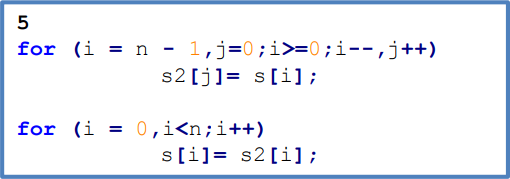
\includegraphics[width=0.7\textwidth]{Abigail/Ejercicio09/Images/5.PNG}
    \end{figure} 

    \subsection{Dijkstra}

      \subsubsection{Tabla}
        Ruta más corta desde el nodo 1 hasta los demás.

        \begin{itemize}
          \item La ruta más costosa: 14 hacia el nodo 14.
        \end{itemize}

       \begin{figure}[h!]
          \centering
          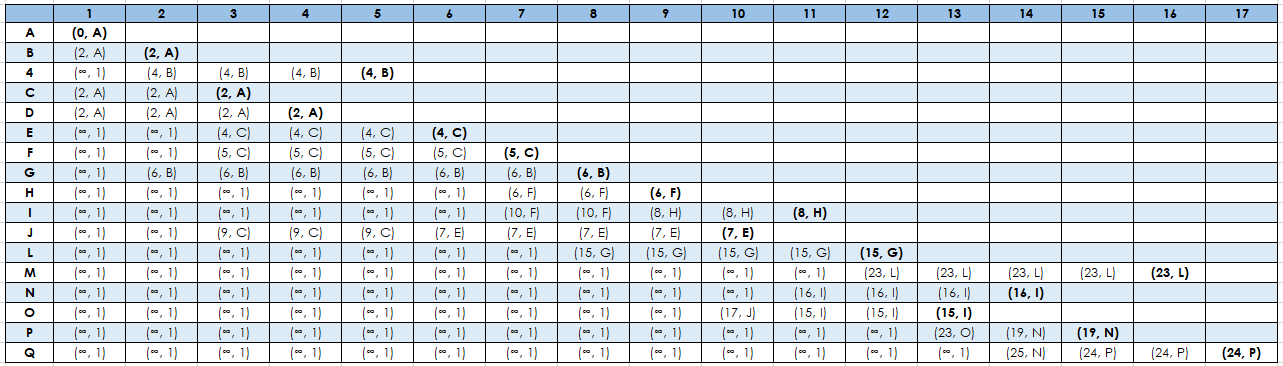
\includegraphics[width=0.7\textwidth]{Abigail/Ejercicio09/Images/5_DT.PNG}
        \end{figure} 

      \subsubsection{Resultado}
        \begin{figure}[h!]
          \centering
          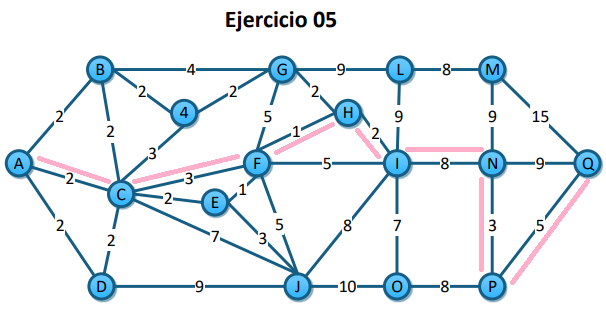
\includegraphics[width=0.7\textwidth]{Abigail/Ejercicio09/Images/5_DR.PNG}
        \end{figure} 

    \subsection{Prim}

      \subsubsection{Explicación}

      \subsubsection{Tabla}

      \subsubsection{Resultado}

    \subsection{Kruskal}

      \subsubsection{Explicación}

      \subsubsection{Tabla}

      \subsubsection{Resultado}

\end{document}